\documentclass[11pt,a4paper]{article}

\usepackage[a4paper,margin=22mm,headheight=24pt]{geometry}
\usepackage{amsmath,amssymb}
\usepackage{array,booktabs,tabularx}
\usepackage{xcolor}
\usepackage{enumitem}
\usepackage{fancyhdr}
\usepackage{listings}
\usepackage{graphicx}
\usepackage{microtype}
\usepackage{hyperref}

\definecolor{navy}{HTML}{17324D}
\definecolor{teal}{HTML}{087E8B}
\definecolor{pale}{HTML}{EEF5F7}
\definecolor{codebg}{HTML}{F4F6F8}

\hypersetup{colorlinks=true,linkcolor=navy,urlcolor=teal}
\setlength{\parindent}{0pt}
\setlength{\parskip}{4pt}
\setlist{nosep,leftmargin=*}
\renewcommand{\arraystretch}{1.18}

\lstset{
  language=Matlab,
  basicstyle=\ttfamily\small,
  columns=fullflexible,
  keepspaces=true,
  frame=single,
  framerule=0.4pt,
  rulecolor=\color{gray!45},
  backgroundcolor=\color{codebg},
  showstringspaces=false,
  aboveskip=5pt,
  belowskip=5pt
}

\pagestyle{fancy}
\fancyhf{}
\lhead{\textcolor{navy}{PHY4605 Computational Physics}}
\rhead{\textcolor{navy}{Sample Test 1}}
\cfoot{\thepage}
\renewcommand{\headrulewidth}{0.5pt}
\renewcommand{\headrule}{\hbox to\headwidth{\color{teal}\leaders\hrule height \headrulewidth\hfill}}
\makeatletter
\let\ps@plain\ps@fancy
\makeatother

\newcommand{\qmarks}[1]{\hfill\mbox{\textbf{[#1 marks]}}}
\newcommand{\questiontitle}[1]{\vspace{5pt}{\large\color{navy}\textbf{#1}}\par\vspace{2pt}}

\begin{document}

\begin{center}
  {\LARGE\color{navy}\textbf{PHY4605 Computational Physics}}\\[4pt]
  {\Large\color{teal}\textbf{SAMPLE TEST 1}}\\[4pt]
  {\large From Physical Model to Checkable Computation}
\end{center}

\vspace{4pt}
\begin{tabularx}{\textwidth}{@{}>{\bfseries}l X >{\bfseries}l X@{}}
  Course weight: & 10\% & Time: & 90 minutes \\
  Mode: & Individual, open-book, AI-free & Raw marks: & 50
\end{tabularx}

\vspace{6pt}
\fcolorbox{teal}{pale}{\parbox{0.96\textwidth}{\textbf{Sample only.} This paper is a format and scope example for discussion. It is not an official assessment paper.}}

\section*{Instructions}
\begin{itemize}
  \item Use the supplied formulas and reference box. Open-book means that approved course notes and reference material may be consulted; generative-AI assistance, collaboration, and answer sharing are not permitted.
  \item MATLAB execution is not required. Where a code fragment is supplied, reason from the code and the physical model.
  \item Show enough working for another reader to follow your model, units, algorithm, validation, and physical interpretation.
  \item Use \(g=9.81\ \mathrm{m\,s^{-2}}\) unless a question states otherwise. Give numerical answers with sensible units and precision.
  \item Short pseudocode is sufficient. Do not write a complete program from a blank page.
\end{itemize}

\section*{Compact reference box}
\begin{align*}
  E(r) &= \frac{k_e Q}{r^2},
  \qquad k_e=8.99\times10^9\ \mathrm{N\,m^2\,C^{-2}},\\
  H(v_0,\theta) &= \frac{v_0^2\sin^2\theta}{2g},\\
  \begin{bmatrix}a&b&0\\b&c&d\\0&d&e\end{bmatrix}
  \begin{bmatrix}I_1\\I_2\\I_3\end{bmatrix}
  &= \begin{bmatrix}s_1\\s_2\\s_3\end{bmatrix},\\
  R(\theta) &= \frac{v_0^2}{g}\sin(2\theta),
  \qquad f(\theta)=R(\theta)-R_{\mathrm{target}}.
\end{align*}
For array calculations in MATLAB, use element-wise operators such as \texttt{.*}, \texttt{./}, and \texttt{.\textasciicircum}. MATLAB indexing starts at 1.

\questiontitle{Question 1 - Transfer an array model to a field problem}

A point charge \(Q=3.0\ \mathrm{nC}\) is fixed at the origin. The magnitude of its electric field is sampled along a radial line at
\(r=0.10,0.20,0.30,0.40,0.50\ \mathrm{m}\). The radial direction away from the charge is taken as positive.

\textbf{(a)} Complete the table. \qmarks{4}

\begin{center}
\begin{tabularx}{0.9\textwidth}{@{}>{\raggedright\arraybackslash}p{0.2\textwidth} X >{\raggedright\arraybackslash}p{0.2\textwidth}@{}}
\toprule
Quantity & Physical meaning & SI unit \\
\midrule
\(Q\) & & \\
\(r\) & & \\
\(k_e\) & & \\
\(E(r)\) & & \\
\bottomrule
\end{tabularx}
\end{center}

\textbf{(b)} Calculate the field magnitude \(E(0.20\ \mathrm{m})\). \qmarks{2}

\textbf{(c)} The following line is intended to calculate the field for every entry in \texttt{r\_m}. Rewrite only the line so the operations are applied element by element. \qmarks{3}

\begin{lstlisting}
E_N = ke_Nm2C2*Q_C/r_m^2;
\end{lstlisting}

\textbf{(d)} Before viewing a supplied plot of \(E\) against \(r\), state the trend you predict and explain why \(r=0\) must not be included in this model. \qmarks{3}

\begin{center}
  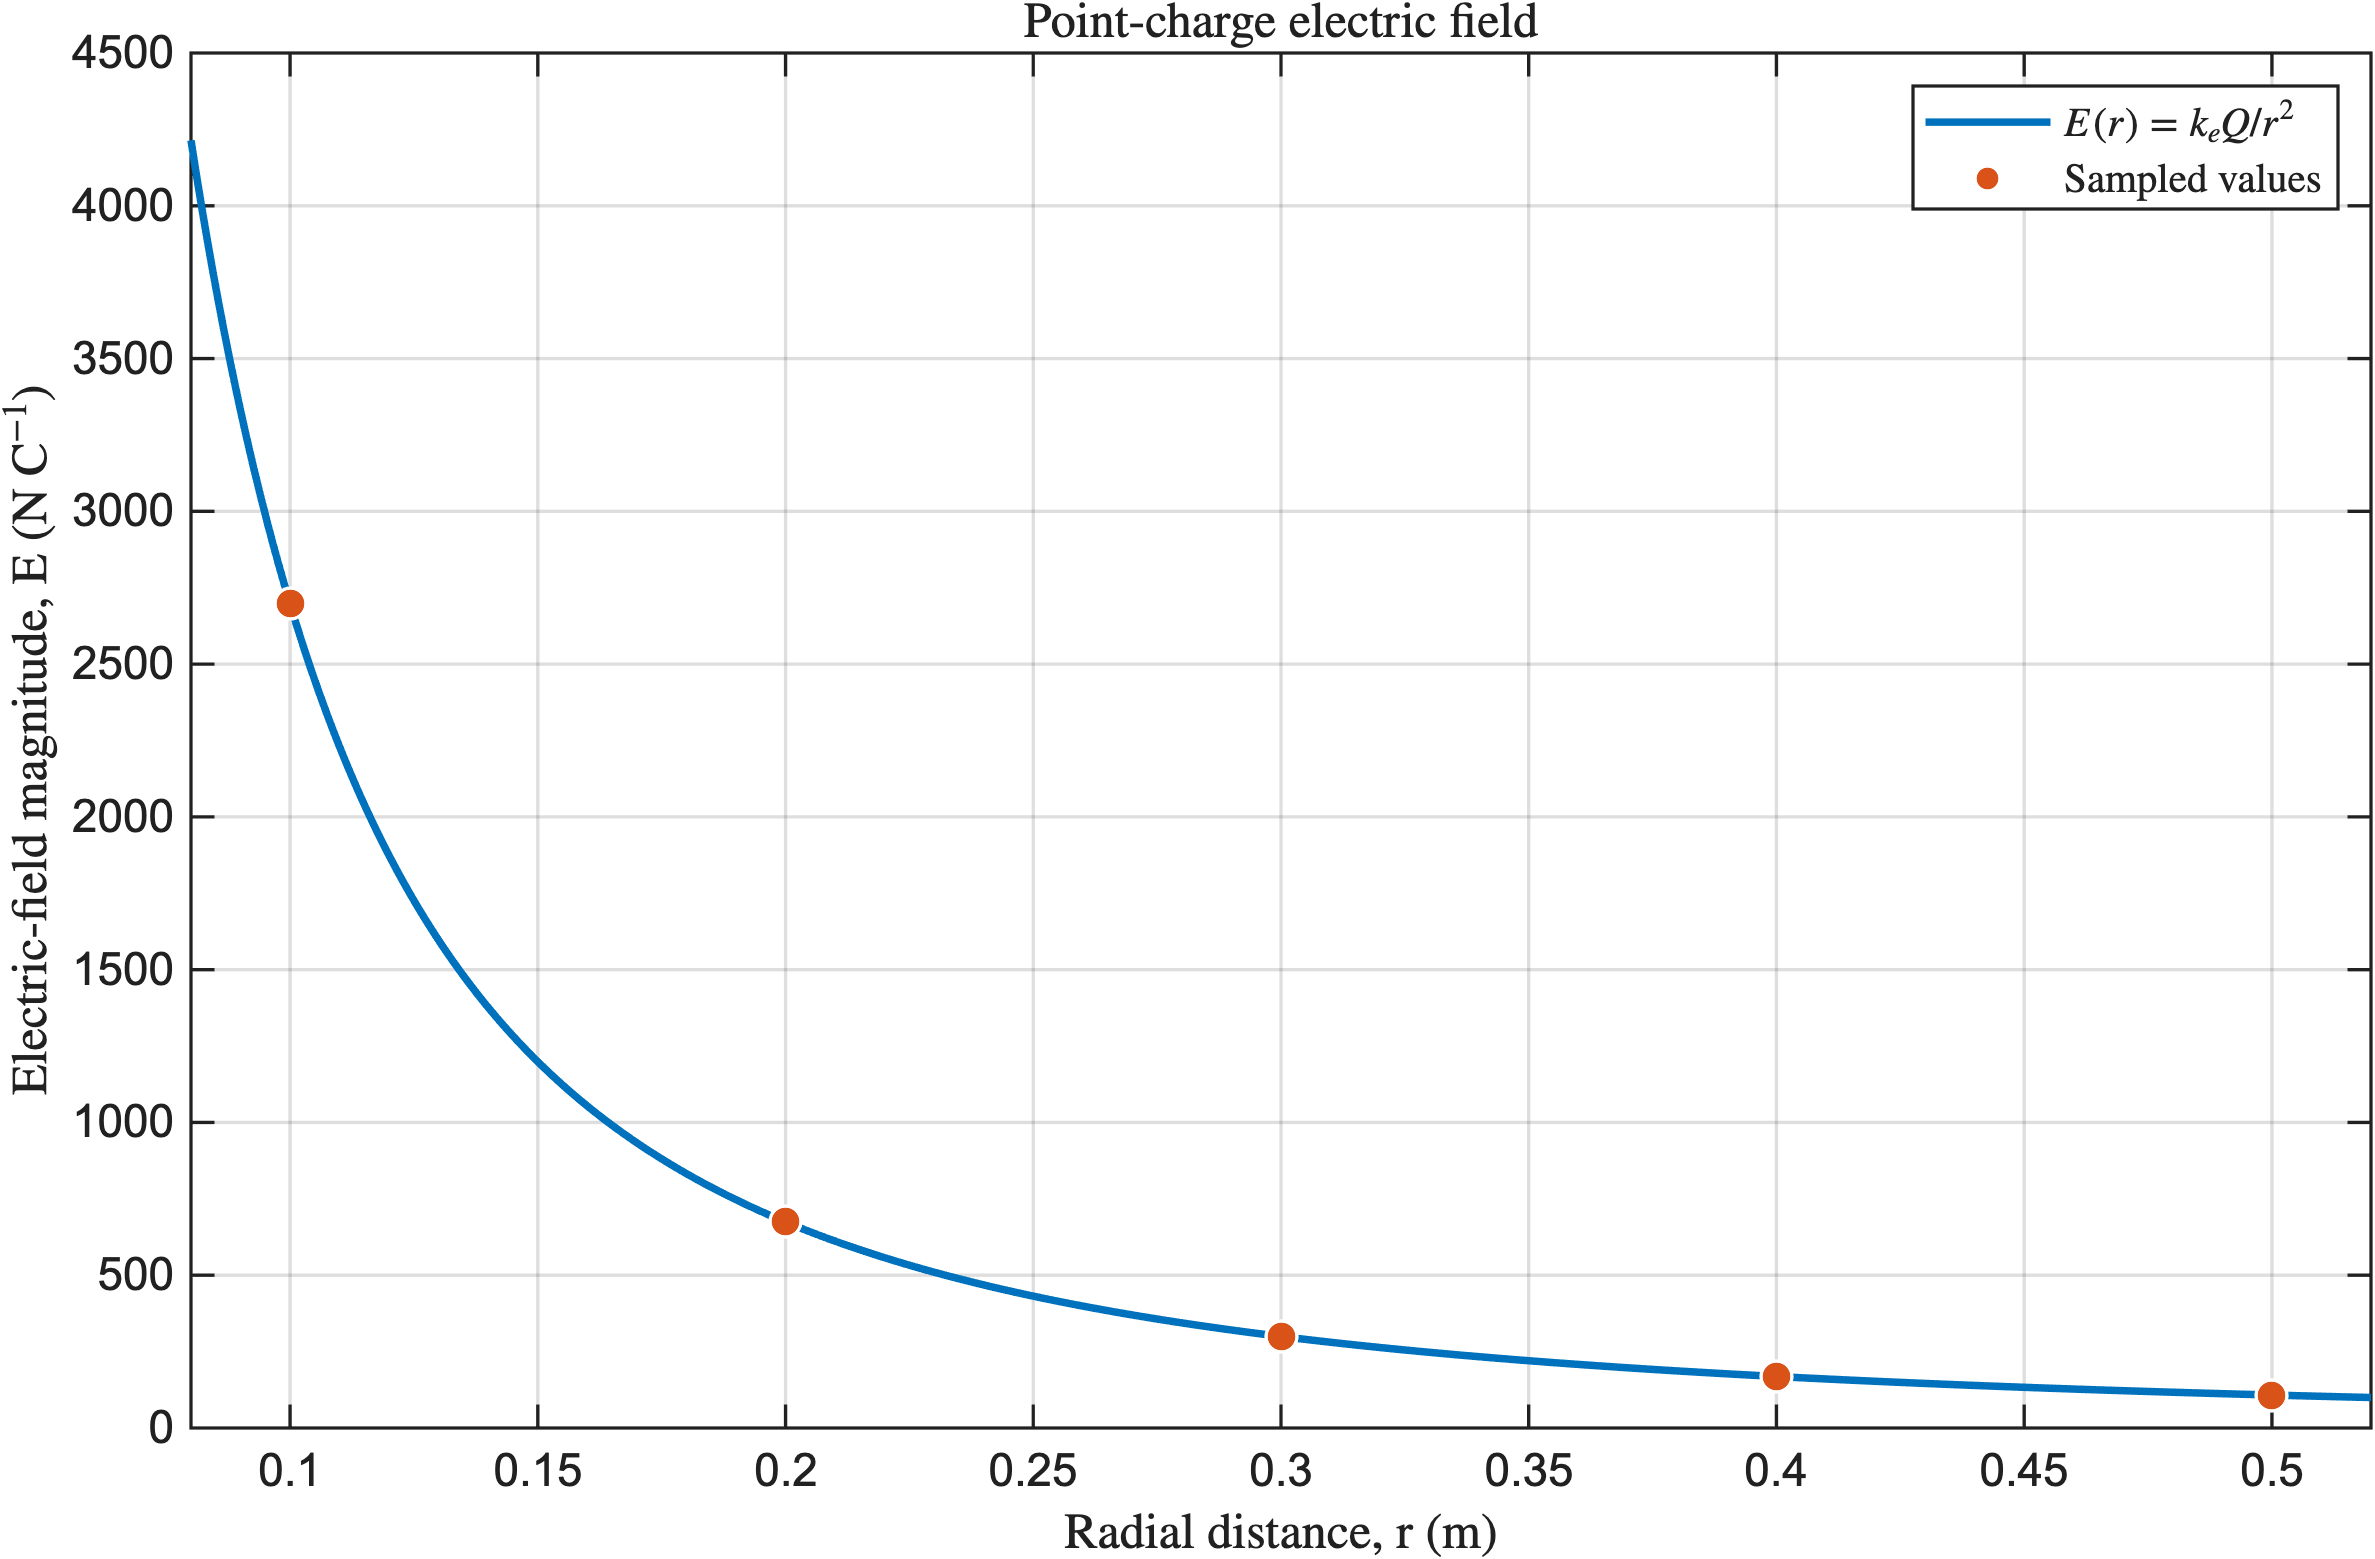
\includegraphics[width=0.82\textwidth]{figures/q1_electric_field_vs_distance.png}\\[-2pt]
  {\small\textit{Figure 1. Supplied electric-field magnitude against radial distance.}}
\end{center}

\textbf{(e)} A student writes the following loop. Identify the defect, describe its consequence for the output array, and give the corrected assignment target. \qmarks{4}

\begin{lstlisting}
ke_Nm2C2 = 8.99e9;
Q_C = 3.0e-9;
r_m = 0.10:0.10:0.50;
E_N = zeros(size(r_m));

for sample_index = 1:numel(r_m)
    current_r_m = r_m(sample_index);
    E_N(1) = ke_Nm2C2*Q_C/current_r_m^2;
end
\end{lstlisting}

\textbf{Total for Question 1: 16 marks}

\newpage
\questiontitle{Question 2 - Assemble and solve a three-loop Kirchhoff system}

A circuit schematic with three clockwise mesh currents, \(I_1\), \(I_2\), and \(I_3\), is shown below. The voltage-source polarity is marked on the diagram. A resistor shared by two meshes carries the difference of the corresponding mesh currents. The KVL equations obtained from the stated clockwise convention are supplied after the diagram.

\begin{center}
{\setlength{\unitlength}{1mm}
\begin{picture}(150,69)
  % outer and shared vertical branches
  \put(5,57){\line(0,-1){13}}
  \put(5,28){\line(0,-1){13}}
  \put(52,57){\line(0,-1){13}}
  \put(52,28){\line(0,-1){13}}
  \put(99,57){\line(0,-1){13}}
  \put(99,28){\line(0,-1){13}}
  \put(146,57){\line(0,-1){13}}
  \put(146,28){\line(0,-1){13}}
  % vertical resistors
  \put(-1,28){\framebox(12,16){\scriptsize\shortstack{$R_1$\\$2\,\Omega$}}}
  \put(46,28){\framebox(12,16){\scriptsize\shortstack{$R_3$\\$1\,\Omega$}}}
  \put(93,28){\framebox(12,16){\scriptsize\shortstack{$R_5$\\$1\,\Omega$}}}
  \put(140,28){\framebox(12,16){\scriptsize\shortstack{$R_7$\\$2\,\Omega$}}}
  % top resistors and connecting wires
  \put(5,57){\line(1,0){8}}
  \put(39,57){\line(1,0){13}}
  \put(52,57){\line(1,0){8}}
  \put(86,57){\line(1,0){13}}
  \put(99,57){\line(1,0){8}}
  \put(133,57){\line(1,0){13}}
  \put(13,53){\framebox(26,8){\scriptsize$R_2=3\,\Omega$}}
  \put(60,53){\framebox(26,8){\scriptsize$R_4=2\,\Omega$}}
  \put(107,53){\framebox(26,8){\scriptsize$R_6=4\,\Omega$}}
  % bottom voltage sources and connecting wires
  \put(5,15){\line(1,0){17.5}}
  \put(34.5,15){\line(1,0){17.5}}
  \put(52,15){\line(1,0){17.5}}
  \put(81.5,15){\line(1,0){17.5}}
  \put(99,15){\line(1,0){17.5}}
  \put(128.5,15){\line(1,0){17.5}}
  \put(28.5,15){\circle{12}}
  \put(75.5,15){\circle{12}}
  \put(122.5,15){\circle{12}}
  \put(25.5,15){\makebox(0,0){\scriptsize$+$}}
  \put(31.5,15){\makebox(0,0){\scriptsize$-$}}
  \put(72.5,15){\makebox(0,0){\scriptsize$+$}}
  \put(78.5,15){\makebox(0,0){\scriptsize$-$}}
  \put(119.5,15){\makebox(0,0){\scriptsize$+$}}
  \put(125.5,15){\makebox(0,0){\scriptsize$-$}}
  \put(28.5,3){\makebox(0,0){\scriptsize$V_1=12\,\mathrm{V}$}}
  \put(75.5,3){\makebox(0,0){\scriptsize$V_2=6\,\mathrm{V}$}}
  \put(122.5,3){\makebox(0,0){\scriptsize$V_3=9\,\mathrm{V}$}}
  % mesh-current markers
  \put(28.5,37){\makebox(0,0){\Large$\circlearrowright$}}
  \put(28.5,30){\makebox(0,0){\scriptsize$I_1$}}
  \put(75.5,37){\makebox(0,0){\Large$\circlearrowright$}}
  \put(75.5,30){\makebox(0,0){\scriptsize$I_2$}}
  \put(122.5,37){\makebox(0,0){\Large$\circlearrowright$}}
  \put(122.5,30){\makebox(0,0){\scriptsize$I_3$}}
\end{picture}}
\end{center}

\begin{align*}
  (R_1+R_2+R_3)I_1-R_3I_2 &= V_1,\\
  -R_3I_1+(R_3+R_4+R_5)I_2-R_5I_3 &= V_2,\\
  -R_5I_2+(R_5+R_6+R_7)I_3 &= V_3.
\end{align*}

\textbf{(a)} Identify the three unknowns and state their units. Explain why the coefficients coupling neighbouring mesh currents are negative. \qmarks{3}

\textbf{(b)} Write the numerical matrix equation \(A\mathbf{I}=\mathbf{b}\), including units for the current vector and source-vector entries. \qmarks{4}

\textbf{(c)} Complete the two missing MATLAB statements in the supplied scaffold. Line breaks inside the matrix statement are allowed. \qmarks{3}

\begin{lstlisting}
R1_Ohm = 2; R2_Ohm = 3; R3_Ohm = 1;
R4_Ohm = 2; R5_Ohm = 1; R6_Ohm = 4; R7_Ohm = 2;
V1_V = 12; V2_V = 6; V3_V = 9;

% Assemble the coefficient matrix and source vector.
A = ____________________________________________;
b = ____________________________________________;

% The supplied solve line is not being assessed for memorisation.
I_A = A\b;
\end{lstlisting}

\textbf{(d)} Use the 3$\times$3 matrix equation to calculate \(I_1\), \(I_2\), and \(I_3\) to two decimal places. State the direction of each current relative to the arrows in the diagram. \qmarks{4}

\textbf{(e)} Verify the first KVL equation by direct substitution using your rounded currents. Then calculate the current through the shared resistor \(R_3\) in the direction of \(I_1\) and interpret its sign. \qmarks{2}

\textbf{Total for Question 2: 16 marks}

\newpage
\questiontitle{Question 3 - Compare one controlled change and verify a physical root}

\textbf{Part A: controlled parameter sweep}

For a projectile launched at \(45^\circ\), the maximum height is evaluated for several initial speeds. The angle, \(g\), and model assumptions are held fixed.

\begin{center}
\begin{tabular}{@{}ccc@{}}
\toprule
\(v_0\ (\mathrm{m\,s^{-1}})\) & Maximum height \(H\ (\mathrm{m})\) & \texttt{H} from the supplied computation \\
\midrule
10 & 2.55 & 2.55 \\
15 & 5.73 & 5.73 \\
20 & 10.19 & 10.19 \\
\bottomrule
\end{tabular}
\end{center}

\begin{center}
  \begin{minipage}{0.48\textwidth}
    \centering
    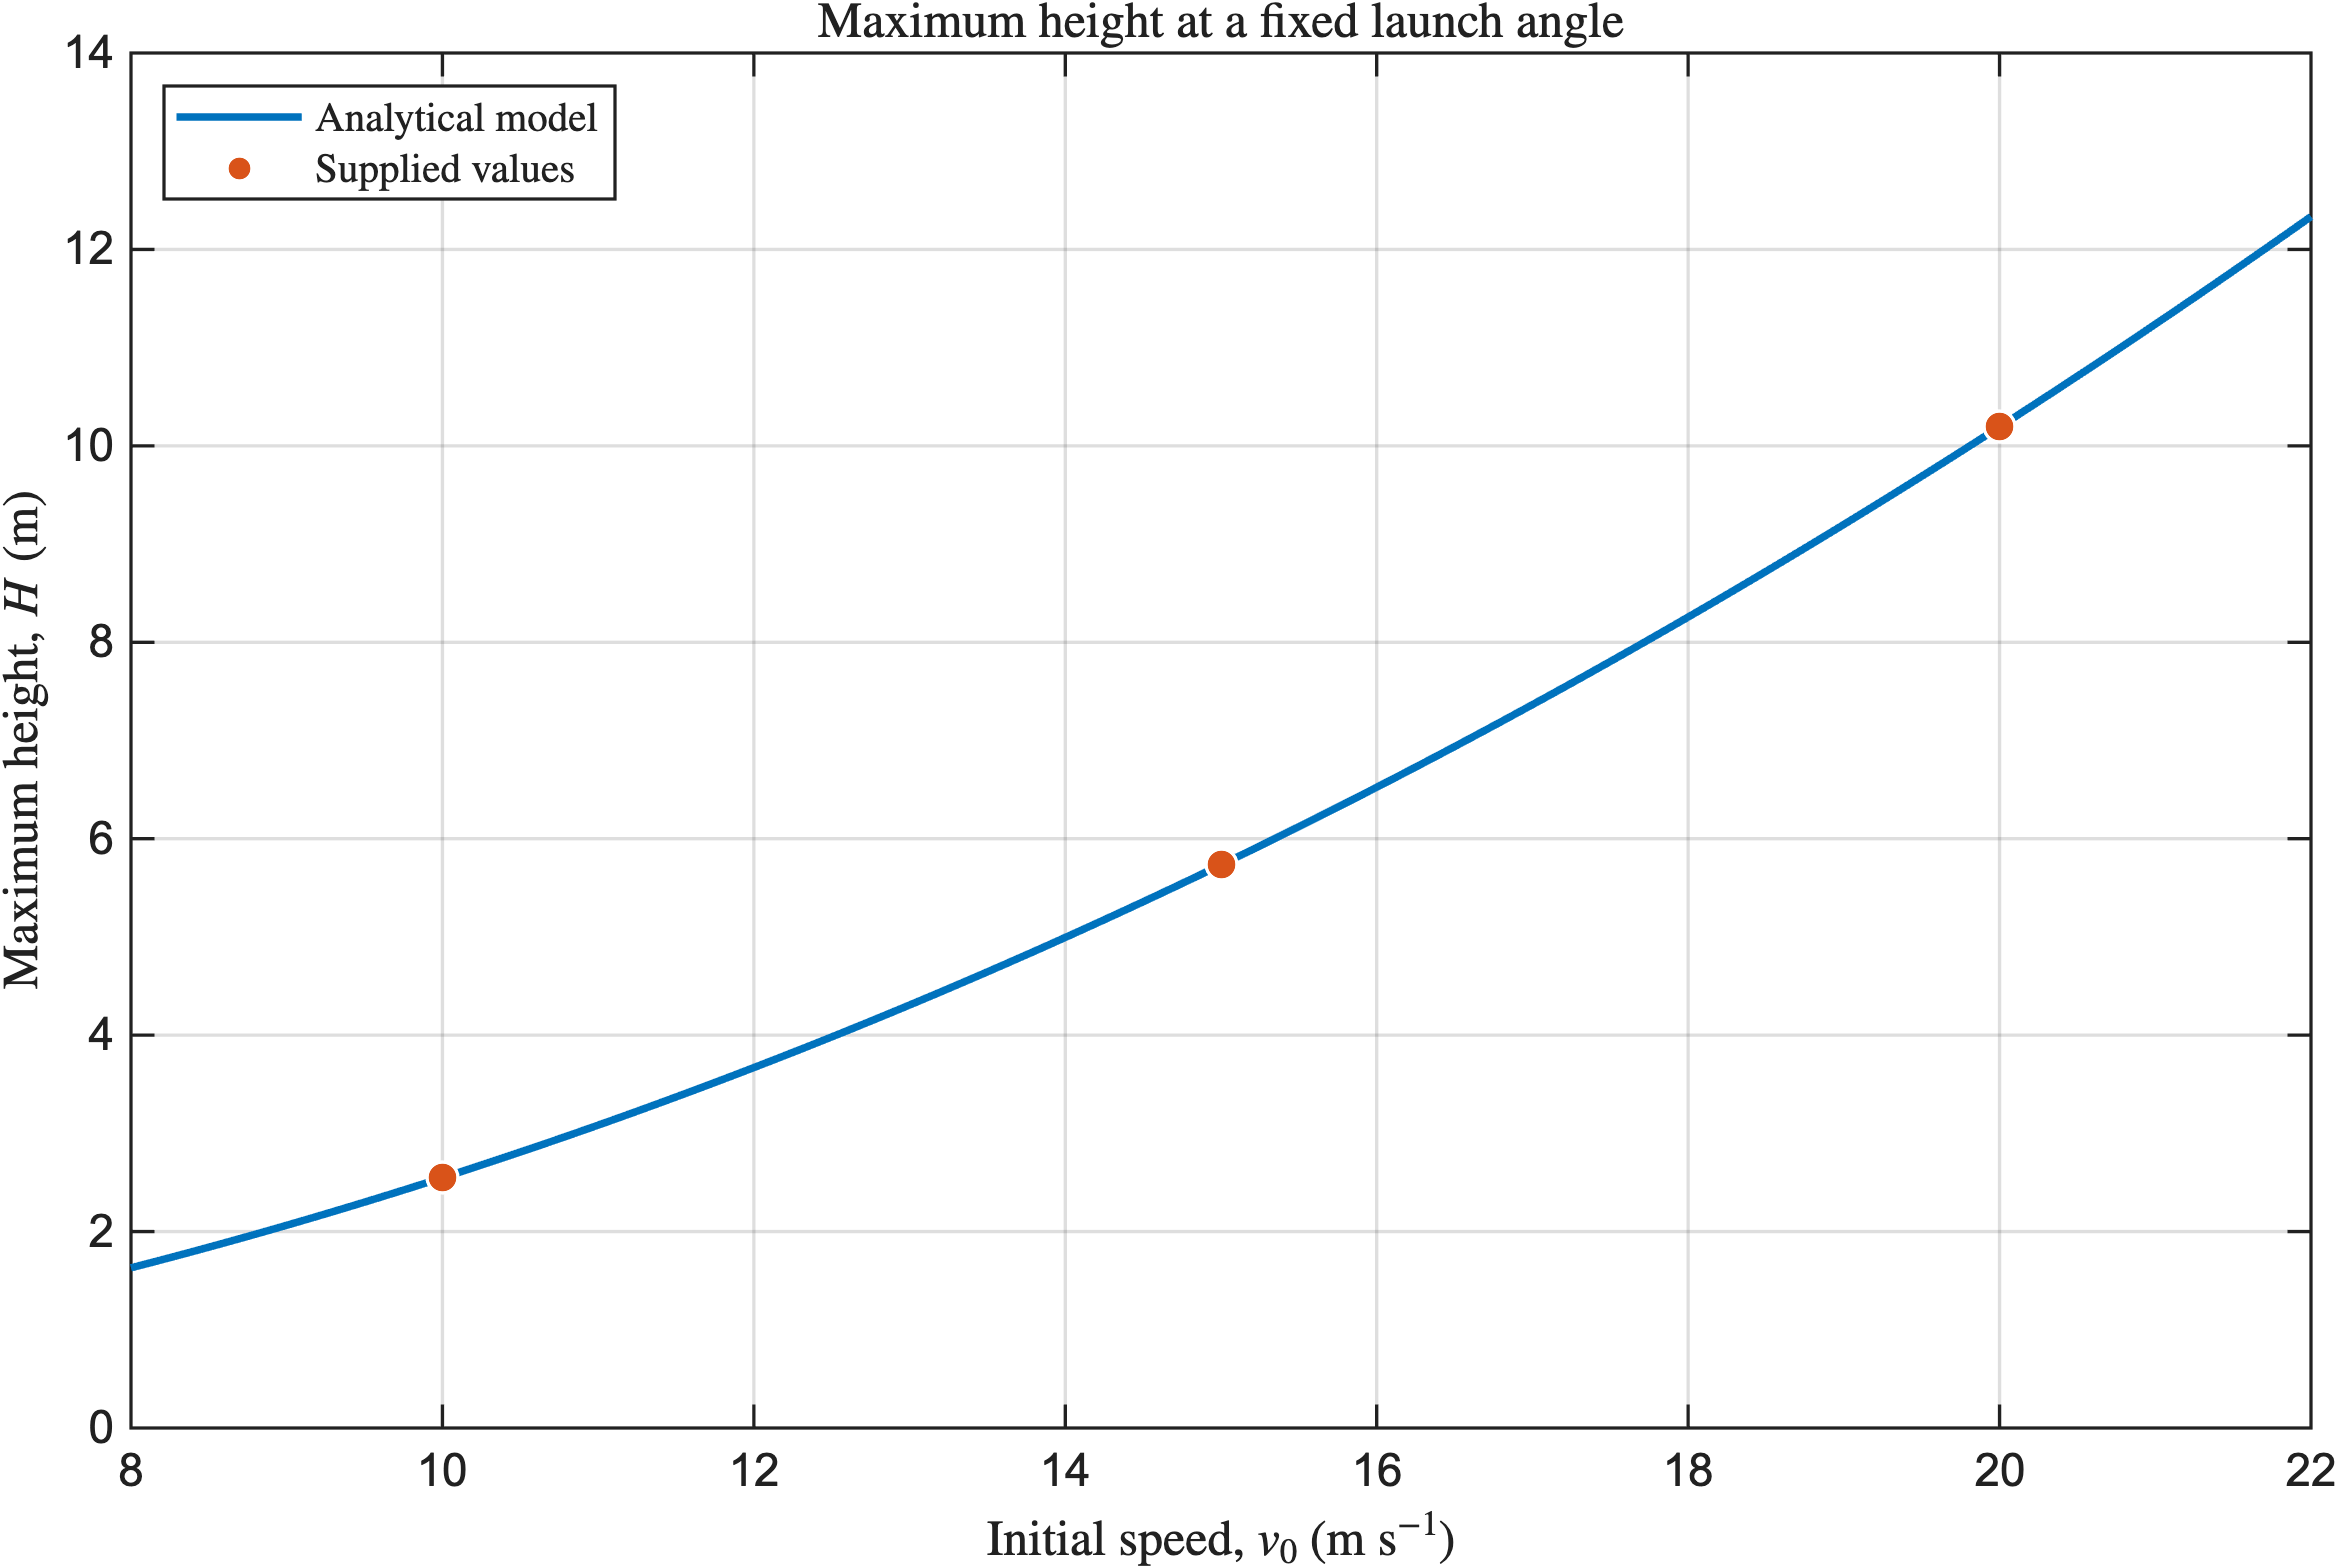
\includegraphics[width=\textwidth]{figures/q3_height_vs_initial_speed.png}\\[-2pt]
    {\small\textit{Figure 2. Supplied height sweep.}}
  \end{minipage}\hfill
  \begin{minipage}{0.48\textwidth}
    \centering
    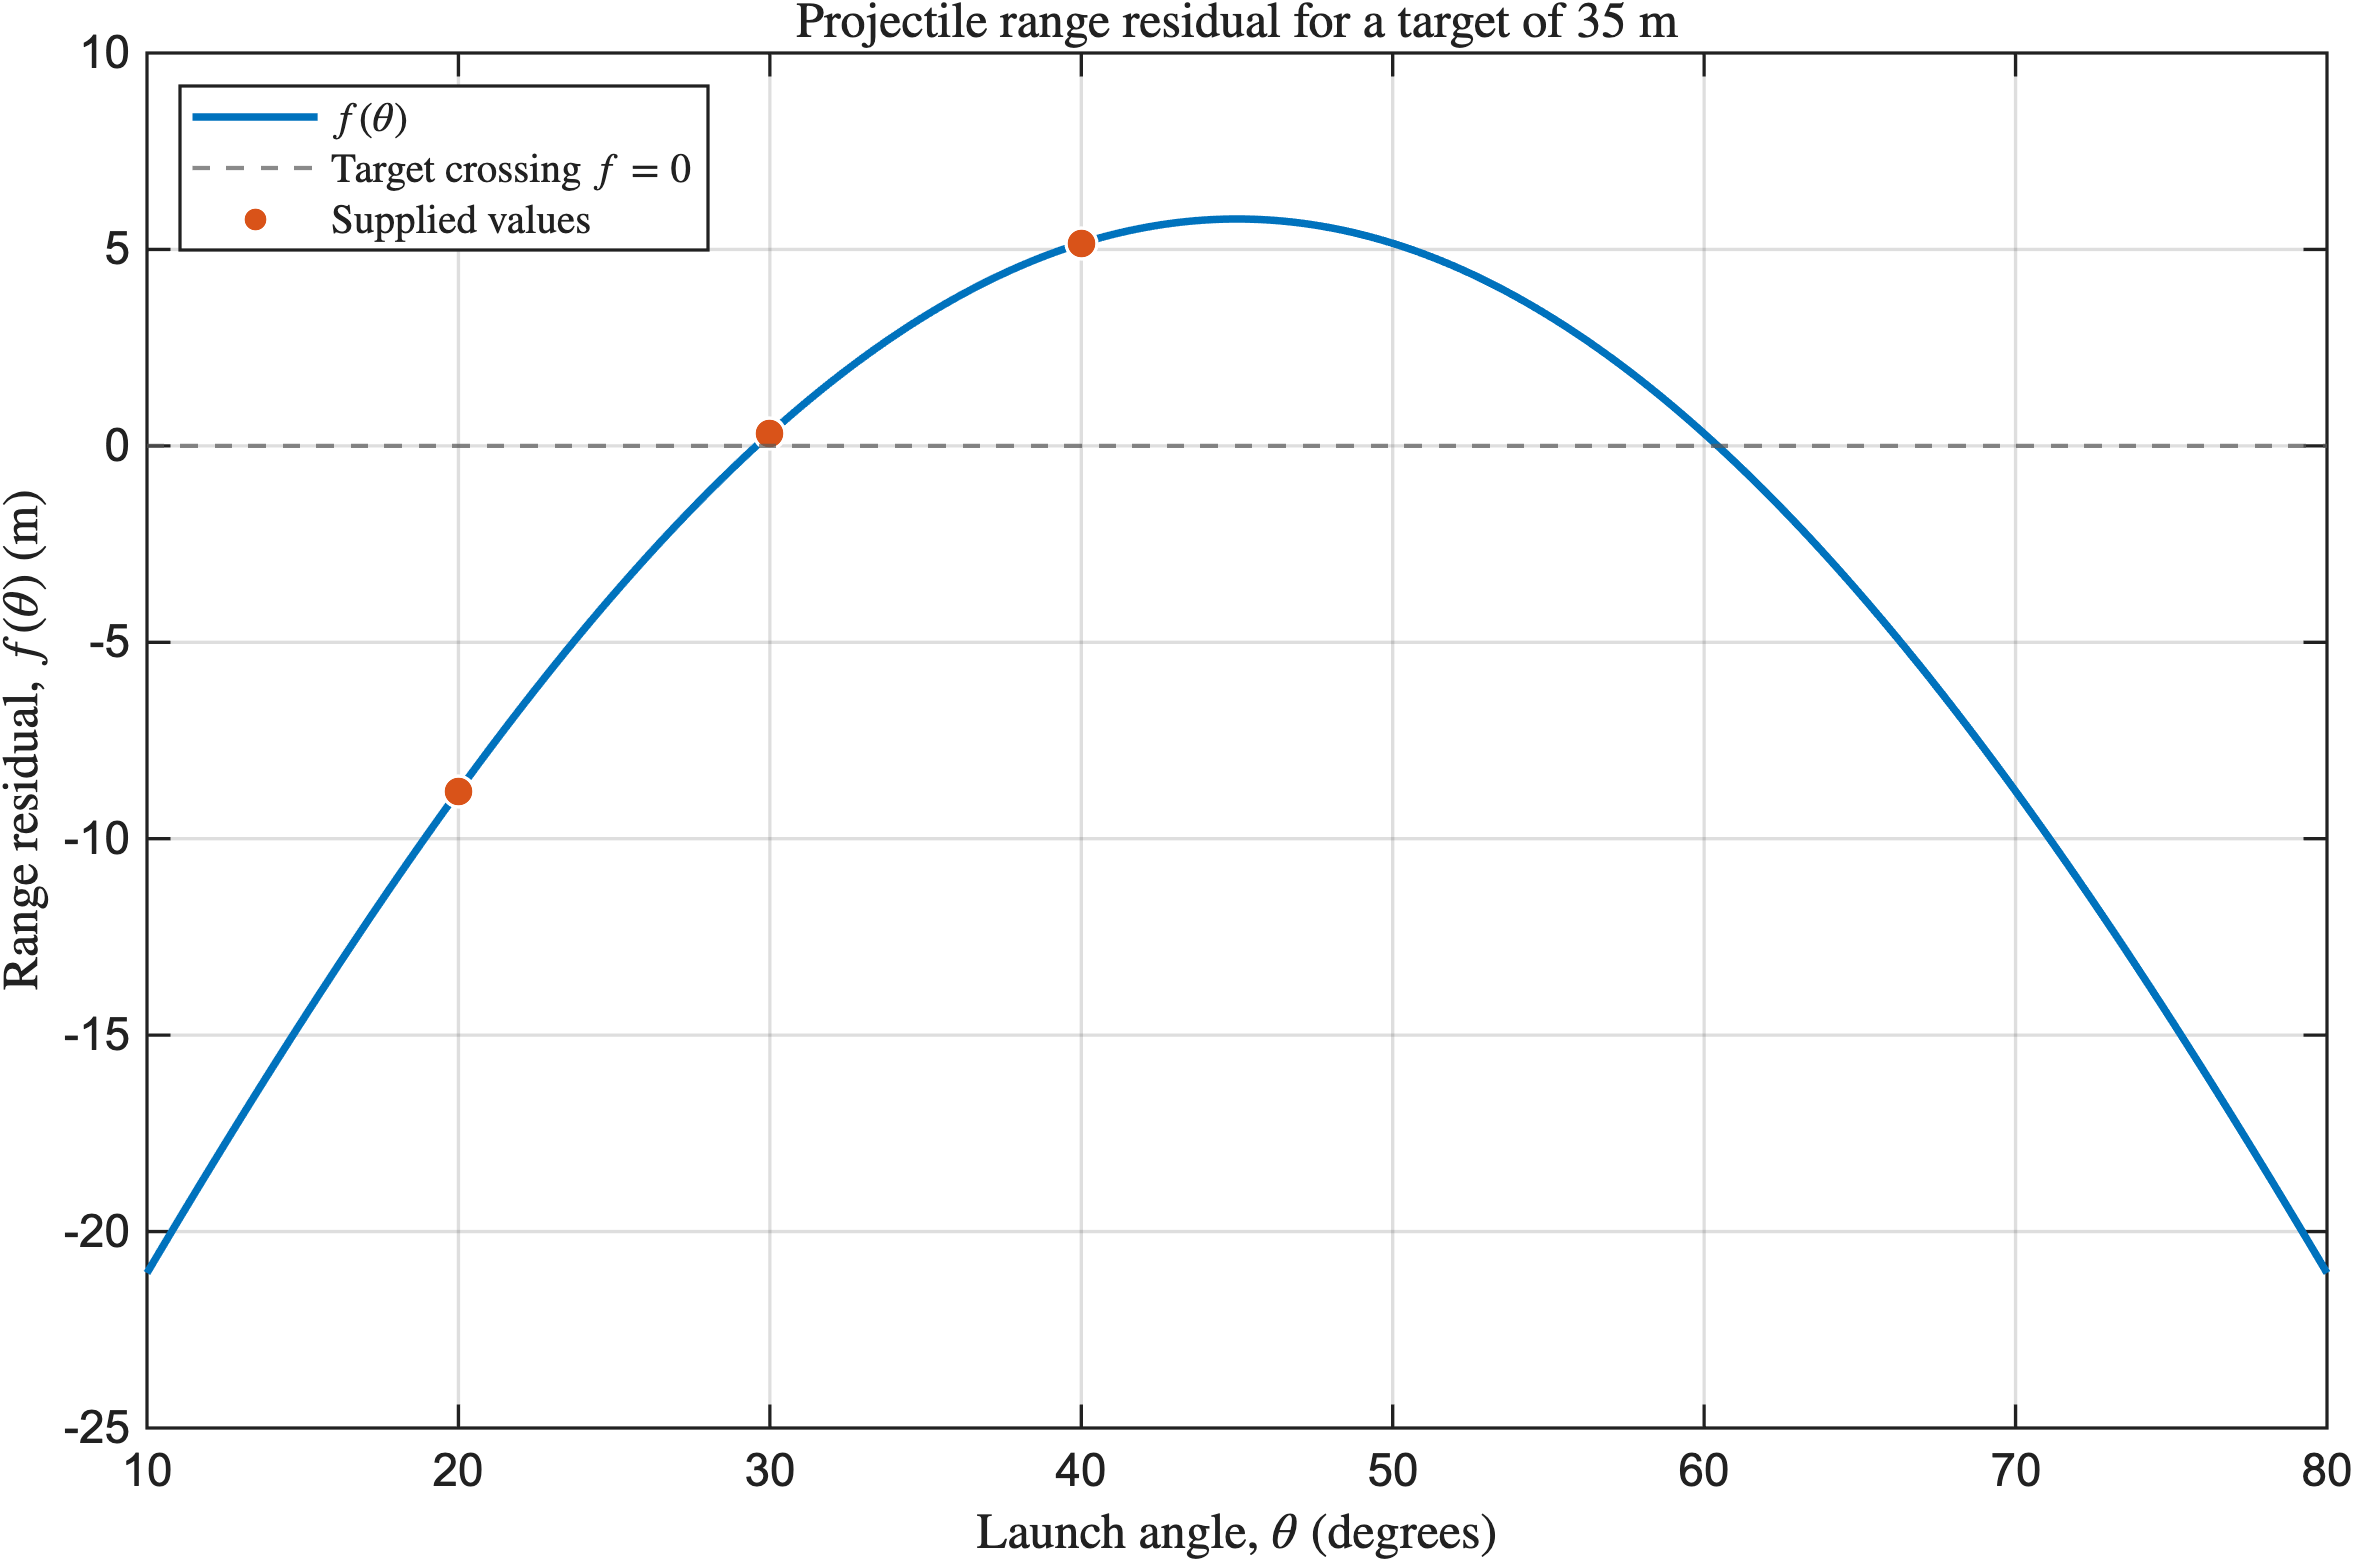
\includegraphics[width=\textwidth]{figures/q3_range_residual_vs_angle.png}\\[-2pt]
    {\small\textit{Figure 3. Supplied residual plot.}}
  \end{minipage}
\end{center}

\textbf{(a)} State which quantity is varied, which quantities are held fixed, and one physical trend supported by the table. \qmarks{3}

\textbf{(b)} Complete the short pseudocode. Use no more than four lines in the answer. \qmarks{3}

\begin{lstlisting}
choose an array of initial speeds v0
for each __________________________________________
    calculate ______________________________________
    store _________________________________________
end
\end{lstlisting}

\textbf{(c)} Give one baseline, limiting-case, or unit check that would help validate this sweep. \qmarks{2}

\textbf{Part B: residual and bisection reasoning}

For a projectile with \(v_0=20\ \mathrm{m\,s^{-1}}\), the target range is \(35\ \mathrm{m}\). The supplied residual values are:

\begin{center}
\begin{tabular}{@{}cccc@{}}
\toprule
Launch angle \(\theta\) & \(20^\circ\) & \(30^\circ\) & \(40^\circ\) \\
\midrule
Residual \(f(\theta)\ (\mathrm{m})\)
  & -8.7905 & +0.3119 & +5.1553 \\
\bottomrule
\end{tabular}
\end{center}

\textit{Use Figure 3 as a graphical cross-check after recording your sign-based bracket.}

\textbf{(d)} Select a sign-changing starting bracket for the low-angle root. Explain what the two signs mean physically. \qmarks{2}

\textbf{(e)} Bisection tests the midpoint \(30^\circ\). What is the next bracket? Explain briefly using the residual signs. \qmarks{2}

\textbf{(f)} A scaffolded solver reports \(\theta=29.5673^\circ\), and direct substitution gives \(R=34.9999946\ \mathrm{m}\). The tolerance is \(10^{-3}\ \mathrm{m}\). Calculate the residual, decide whether the validation passes, and state the physical meaning of the root. \qmarks{4}

\textbf{(g)} State one model limitation and one check other than direct substitution that supports the result. \hfill\textbf{[1 mark]}

\textbf{Total for Question 3: 18 marks}

\vfill
\begin{center}
  \color{teal}\rule{0.75\textwidth}{0.5pt}\\[3pt]
  \small\textit{End of sample paper - check units, algorithm logic, validation, and physical interpretation before submission.}
\end{center}

\newpage
\thispagestyle{fancy}
\begin{center}
  {\LARGE\color{navy}\textbf{Instructor Answer Scheme}}\\[4pt]
  {\large Sample Test 1 - reference only}
\end{center}

\fcolorbox{teal}{pale}{\parbox{0.96\textwidth}{\textbf{Use of this section:} This answer scheme is intentionally included at the end of the same sample PDF for discussion and calibration. It is not part of the student question-paper pages. Award equivalent wording when the physical meaning, units, algorithm, or check is correct.}}

\questiontitle{Question 1 - 16 marks}

\begin{center}
\begin{tabularx}{0.96\textwidth}{@{}>{\raggedright\arraybackslash}p{0.16\textwidth} X >{\raggedright\arraybackslash}p{0.18\textwidth}@{}}
\toprule
Quantity & Expected meaning & SI unit \\
\midrule
\(Q\) & Source charge & \(\mathrm{C}\) \\
\(r\) & Radial distance from the charge & \(\mathrm{m}\) \\
\(k_e\) & Coulomb constant & \(\mathrm{N\,m^2\,C^{-2}}\) \\
\(E(r)\) & Electric-field magnitude at distance \(r\) & \(\mathrm{N\,C^{-1}}\) \\
\bottomrule
\end{tabularx}
\end{center}

\textbf{(b)}
\[
  E(0.20)=\frac{(8.99\times10^9)(3.0\times10^{-9})}{(0.20)^2}
  =674.25\ \mathrm{N\,C^{-1}}.
\]

\textbf{(c)}
\begin{lstlisting}
E_N = ke_Nm2C2.*Q_C./r_m.^2;
\end{lstlisting}
Accept scalar multiplication written with \texttt{*} when the student correctly uses \texttt{./} and \texttt{.\textasciicircum2} for the array operations.

\textbf{(d)} The field magnitude decreases as \(r\) increases, following an inverse-square trend. The point-charge model is singular at \(r=0\), so the source location cannot be included as a finite sampled field value.

\textbf{(e)} The assignment target \texttt{E\_N(1)} overwrites the first array entry on every loop pass. At the end, only the final value remains at index 1 and the other entries are still zero. The corrected target is \texttt{E\_N(sample\_index)}.

\textbf{Mark allocation:} 1 mark per correct table row; 2 for substitution and value with unit; 3 for the element-wise line; 1.5 for the inverse-square trend and 1.5 for excluding \(r=0\); 1 for the defect, 1 for its consequence, and 2 for the corrected target and explanation.

\questiontitle{Question 2 - 16 marks}

\textbf{(a)} The unknowns are the three clockwise mesh currents \(I_1\), \(I_2\), and \(I_3\), all in amperes. A shared-resistor term is proportional to a current difference, for example \(R_3(I_1-I_2)\). When this is collected into the equation for mesh 1, the neighbouring-current coefficient is therefore negative. Award 2 marks for the unknowns and units, and 1 for the physical meaning.

\textbf{(b)}
\[
  \begin{bmatrix}6&-1&0\\-1&4&-1\\0&-1&7\end{bmatrix}
  \begin{bmatrix}I_1\\I_2\\I_3\end{bmatrix}
  =\begin{bmatrix}12\\6\\9\end{bmatrix}.
\]
The entries of \(A\) have units \(\Omega\), the current vector has units \(\mathrm{A}\), and the source vector has units \(\mathrm{V}\). Award 2 marks for the coefficient matrix and 2 for the source vector, ordering, and units.

\textbf{(c)}
\begin{lstlisting}
A = [R1_Ohm + R2_Ohm + R3_Ohm, -R3_Ohm, 0; ...
     -R3_Ohm, R3_Ohm + R4_Ohm + R5_Ohm, -R5_Ohm; ...
     0, -R5_Ohm, R5_Ohm + R6_Ohm + R7_Ohm];
b = [V1_V; V2_V; V3_V];
\end{lstlisting}
Award 1.5 marks per statement. Accept equivalent use of the numerical entries or a column-vector construction for \(\mathbf{b}\).

\textbf{(d)} Solving gives \(I_1=2.42\ \mathrm{A}\), \(I_2=2.52\ \mathrm{A}\), and \(I_3=1.65\ \mathrm{A}\). All three values are positive, so each current flows in the clockwise direction shown. Award 2 marks for the values and 2 for units and direction.

\textbf{(e)} Using the rounded values, the first KVL equation gives
\[
  (2+3+1)(2.42)-1(2.52)=12.00\ \mathrm{V},
\]
which agrees with \(V_1\). The current through \(R_3\) in the direction of \(I_1\) is
\[
  I_{R_3}=I_1-I_2=2.42-2.52=-0.10\ \mathrm{A}.
\]
The negative sign means the actual current is approximately \(0.10\ \mathrm{A}\) opposite to the direction of \(I_1\) on the shared branch. Award 1 mark for the KVL check and 1 for the shared-current interpretation.

\questiontitle{Question 3 - 18 marks}

\textbf{(a)} The varied quantity is \(v_0\). The angle \(45^\circ\), \(g\), and model assumptions are fixed. The table supports the trend that maximum height increases as initial speed increases, with a nonlinear approximately quadratic dependence. Award 1 mark for the varied quantity, 1 for fixed quantities, and 1 for a supported trend.

\textbf{(b)} One acceptable completion is:
\begin{lstlisting}
for each current initial speed v0
    calculate H = v0^2*sind(45)^2/(2*g)
    store H for that speed
end
\end{lstlisting}
Accept equivalent MATLAB-like or plain-language pseudocode. Award 1 mark for iterating over speeds, 1 for the maximum-height calculation, and 1 for storing the paired output.

\textbf{(c)} Accept a unit check, \(v_0=0\Rightarrow H=0\), or the quadratic scaling check that doubling \(v_0\) should multiply \(H\) by four when the angle is fixed.

\textbf{(d-e)} A valid starting bracket is \([20^\circ,40^\circ]\) because the residual changes from negative to positive. Since the midpoint \(30^\circ\) has a positive residual while \(20^\circ\) has a negative residual, the next bracket is \([20^\circ,30^\circ]\). A negative residual means the calculated range is below the target.

\textbf{(f)}
\[
  f(\theta)=34.9999946-35=-5.4\times10^{-6}\ \mathrm{m},
  \qquad |f|=5.4\times10^{-6}\ \mathrm{m}<10^{-3}\ \mathrm{m}.
\]
The validation passes. The root is the low launch angle which gives a range of approximately \(35\ \mathrm{m}\) in the stated ideal model. Award 1 mark for the residual, 1 for the absolute comparison, 1 for the conclusion, and 1 for the physical meaning.

\textbf{(g)} Accept a limitation such as neglect of air resistance, level landing, or constant \(g\), together with a different check such as the original sign-changing bracket, a graph crossing, or a plausible-angle check. Award half a mark for each.

\vfill
\begin{center}
  \color{teal}\rule{0.75\textwidth}{0.5pt}\\[3pt]
  \small\textit{End of instructor answer scheme - sample only.}
\end{center}

\end{document}
